\chapter{Acoustic Echo Retrieval}\label{ch:estimation}
\openepigraph{$[\ldots]$ dicebat Bernardus Carnotensis nos esse quasi nanos gigantium humeris insidentes.}{Giovanni of Salisbury, \textit{Metalogicon (III, 4)}}
\vspace{-2.5em}
\newthought{Synopsis}\synopsisChEstimation

\section{Problem formulation}\label{sec:estimation:problem}
As discussed in~\cref{subsec:processing:mixing}, the continuous-time multi-channel signal model for one source signal $\tildes(t)$ and $I$ channels writes, for each channel $\idxMic$,
\begin{equation}\label{eq:estimation:signalmodel}
    \begin{aligned}
        \tildex_i(t) &= (h_i \convCont \tildes)(t) + \tilden_i(t)\\
        \tildeh_i(t) &= \echoModelTimeSimple{i} + \tilde{\varepsilon}_i(t),
    \end{aligned}
\end{equation}
where $\tildeh_i(t)$ is the echo model for the \RIR/ between the $i$-th channel and the source.
The sum comprises the line-of-sight propagation (direct path) and the earliest $\numEchs$ echoes we want to account for, while the error term $\varepsilon_i(t)$ collects later echoes and the reverberation tail.
This model can be generalized to frequency dependent attention, but it will be not addressed here.

\mynewline
\textsc{The \AERdef/ problem consists} in estimating the echoes' timings $\alltaus{i}$ and attenuations (or gains) $\allalphas{i}$ from multichannel observations $\tilde{x}_i$ of~\cref{eq:estimation:signalmodel}.
Depending on the field of research, the echoes' timings are also known as time delays, Time of Arrival \acs{TOA}, or locations.
\\The term \AER/ is not an established name for this problem and, depending on the field of research and the prior knowledge available, it can be referred to with different names.
In fact \AER/ can be seen as a generalization of \textit{\TOAs/ estimation}, or an instance of \textit{acoustic channel estimation} (or \textit{shaping}), \textit{spike retrieval} and \textit{onset detection} (see following~\cref{subsec:estimation:active_rir}).
As opposed to \AER/, the task of \TOAs/ estimation is only focused in estimating the echoes' timings $\alltaus{i}$.
The only knowledge of \TOAs/ is sufficient for typical applications related to \acf{SSL}~\citeonly{ribeiro2010turning} and \RooGE/~\citeonly{crocco2017uncalibrated}.
\\Moreover, knowing $\alltaus{i}$, the attenuations $\allalphas{i}$ can be estimated in closed-form as showed in~\citeonly{condat2015cadzow}.
\\\TOAs/ estimation is sometimes called \textit{time delays estimation}, when the origin of time is taken \wrt/ the first \TOA/ and not to the time of emission.
Hereafter we will make explicit the distinction between the two.
\\\AER/ may be confused with the \textit{acoustic echo cancellation} (AEC) problem in telecommunication and telephony which refers to the problem of estimating and suppressing feedbacks due to loudspeakers being too close to microphones.\sidenote{
    AEC is a problem of very different nature, amounting to suppress from a mixture a known signal distorted by an unknown filter.
    This will not be further discussed in this thesis
}

\section{Taxonomy of Acoustic Echo Retrieval methods}\label{sec:estimation:taxonomy}

% In general, we can identify four main categories which differ on whether the source signal is known and on whether the estimation of the \RIR/ is performed.

\dichotomy{Active vs. passive approaches}.
\textit{Active} methods assume active scenarios, namely, they use one or more loudspeakers to probe the environment and one or more microphones to record the propagated probe sound.
Therefore, they assume that the source reference signal is known.
They falls into the broader category of \textit{deconvolution problems} since a ``clean'' reference signal is used to \textit{deconvolve} the observed one.
The main advantages of these approaches are twofold.
First, provided a proper probe signal, a good estimation of the \RIR/ can be achieved.
Second, these methods can be used on single-channel recordings.
\\Instead, \textit{passive} approaches use sets of passive sensors to record the sound field.
To decouple the environment from the source, they rely either on prior knowledge about the source signal or by comparing the signals received at two (or more) spatially-separated microphones.
When no prior information is available, they can be seen as \textit{blind problem} and are far more challenging.
In the literature, the term blind is used as opposed to \textit{informed}, accounting the amount of prior information available.
With this taxonomy, the above active methods are informed by the exact knowledge of the reference signal.
On the contrary, passive methods need to rely on other general type of information such as sparsity, nonnegativity, \etc/.
In general the labels ``'active \vs/ passive'' apply to the scenario, while ``informed \vs/ blind'' to the problem.
Passive scenarios are more common in real applications and are sometimes preferable to active ones as they are non-intrusive since only already existing sounds are used in the estimation.
Therefore, a great deal of efforts has been devoted to these problems and research is still active in topic.
% The latter is more challenging since, in general settings, theoretical ambiguities make this problem unsolvable~\citeonly{xu1995least, subramaniam1996cepstrum, tong1998multichannel}.

\begin{figure}[h]
    \begin{sidecaption}[Active and passive apporaches]{%
        Schematic view of active \vs/ passive approaches.
    }[fig:estimation:activepassive]
    \centering
    \resizebox{\linewidth}{!}{
        

\tikzset{every picture/.style={line width=0.75pt}} %set default line width to 0.75pt

\begin{tikzpicture}[x=0.75pt,y=0.75pt,yscale=-1,xscale=1]
%uncomment if require: \path (0,300); %set diagram left start at 0, and has height of 300

%Image [id:dp45389501264602794]
\draw (280,131.28) node  {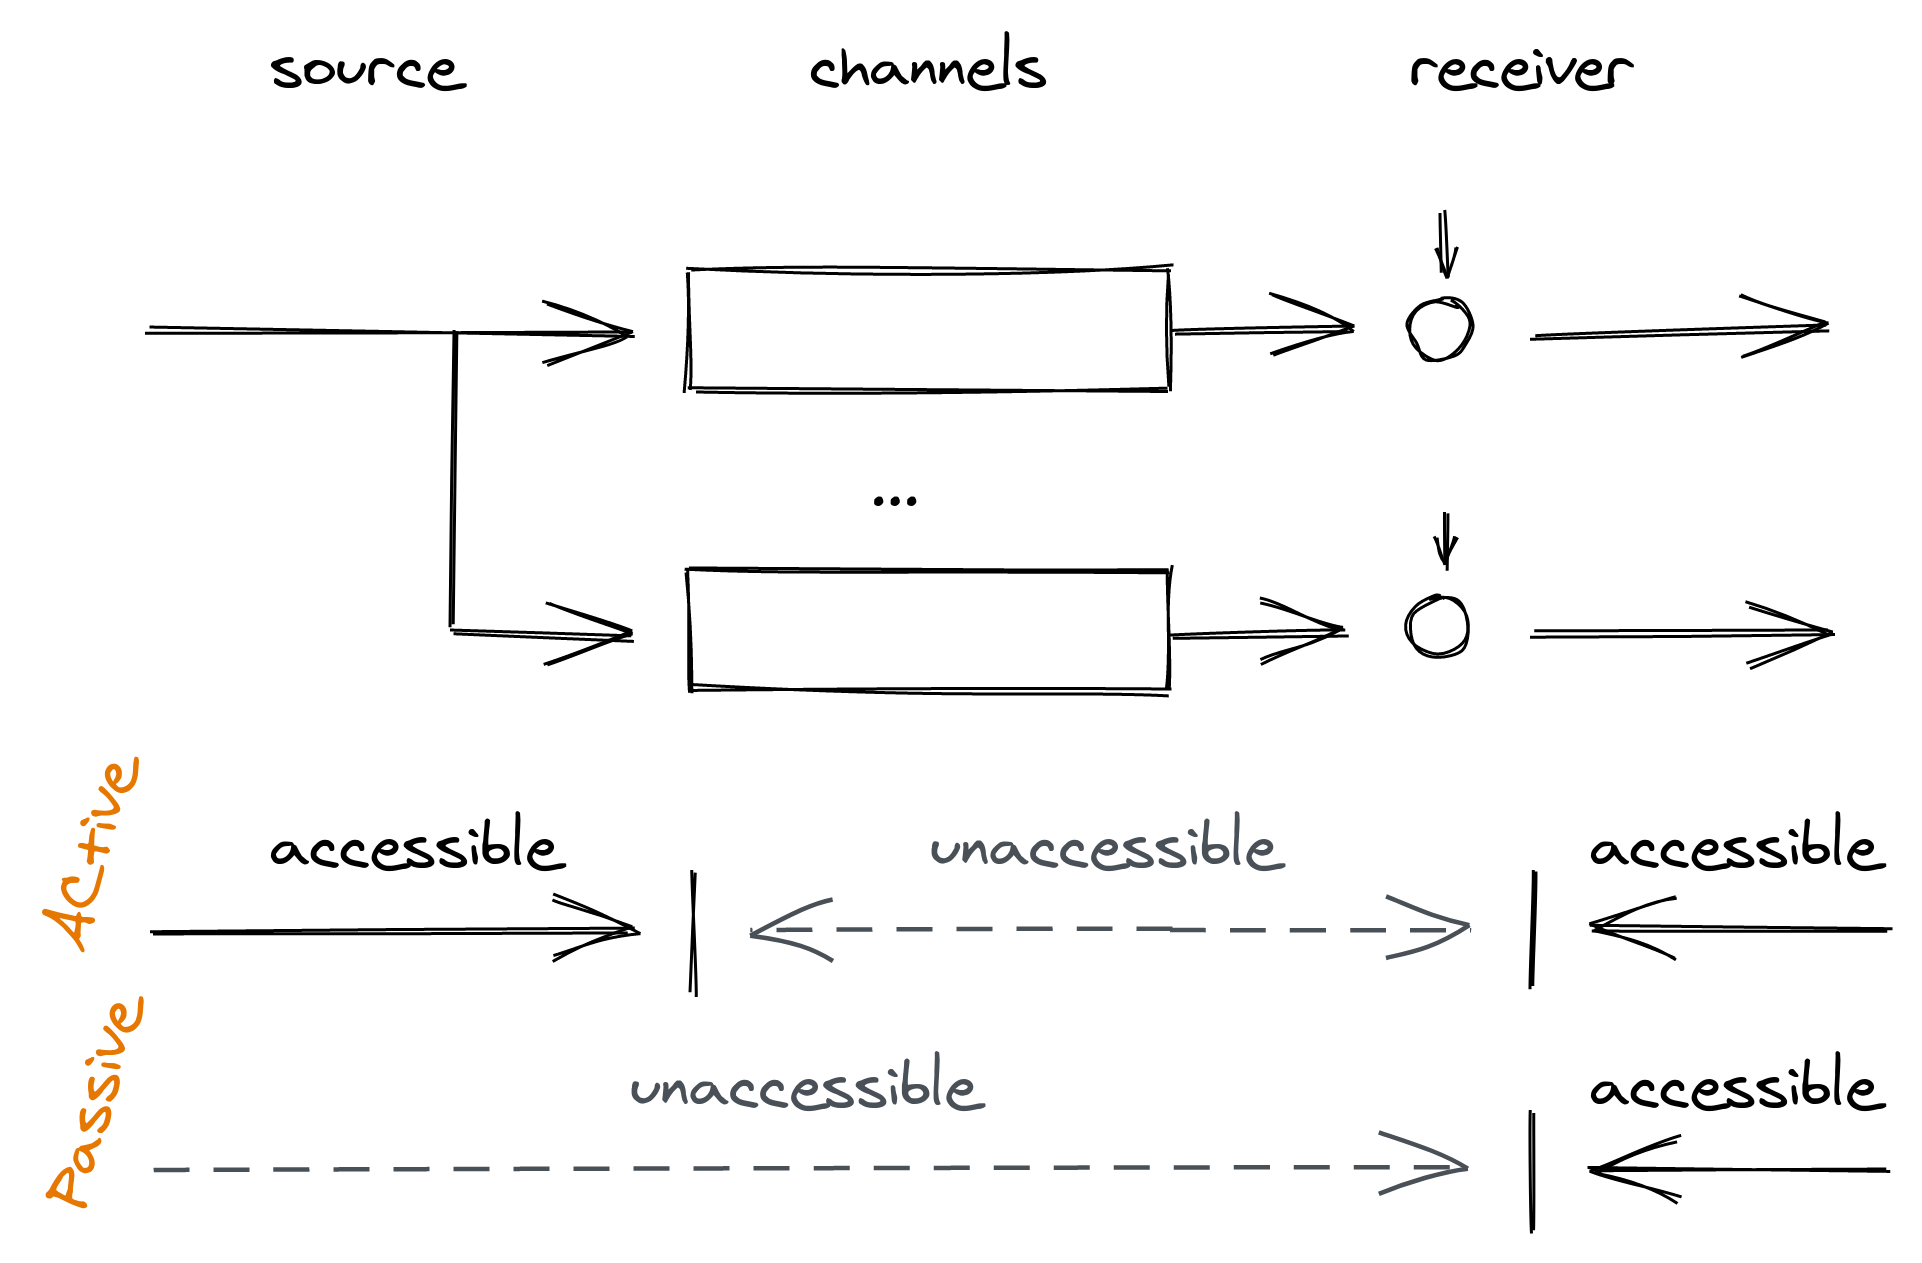
\includegraphics[width=270pt,height=184.92pt]{estimation/ch4_estimation_bce.png}};

% Text Node
\draw (141,54.4) node [anchor=north west][inner sep=0.75pt]  [font=\footnotesize]  {$\tilde{s}( t)$};
% Text Node
\draw (261,60.4) node [anchor=north west][inner sep=0.75pt]  [font=\footnotesize]  {$\tilde{h}_{1}( t)$};
% Text Node
\draw (261,116.4) node [anchor=north west][inner sep=0.75pt]  [font=\footnotesize]  {$\tilde{h}_{I}( t)$};
% Text Node
\draw (432,49.4) node [anchor=north west][inner sep=0.75pt]  [font=\footnotesize]  {$\tilde{x}_{1}( t)$};
% Text Node
\draw (431,109.4) node [anchor=north west][inner sep=0.75pt]  [font=\footnotesize]  {$\tilde{x}_{I}( t)$};
% Text Node
\draw (366.5,33.4) node [anchor=north west][inner sep=0.75pt]  [font=\footnotesize]  {$\tilde{n}_{1}( t)$};
% Text Node
\draw (367.5,86.4) node [anchor=north west][inner sep=0.75pt]  [font=\footnotesize]  {$\tilde{n}_{I}( t)$};
% Text Node
\draw (365,65.4) node [anchor=north west][inner sep=0.75pt]  [font=\footnotesize]  {$+$};
% Text Node
\draw (365,121.4) node [anchor=north west][inner sep=0.75pt]  [font=\footnotesize]  {$+$};


\end{tikzpicture}

    }
    \end{sidecaption}
\end{figure}

\dichotomy{RIR-based vs. RIR-agnostic approches}.
\textit{RIR-based} methods estimate the echoes' properties after estimating the (full or partial) \RIR/(s).
By modeling the early part of the \RIR/ as in~\cref{eq:estimation:signalmodel}, solving the \AER/ problem can be seen as solving two sequential tasks: \RIR/ estimation followed by echo extraction.
The former can be seen as an instance of \textit{channel estimation} (\aka/ \textit{system identification}) problem, while the latter as a \textit{spike retrieval}, \textit{peak picking} or \textit{onset detection} problem.
Other methods estimate the \RIRs/ partially, using assumptions derived by the application.
It is the case of \textit{impulse response shaping} or \textit{shortening}.
In the context of room acoustics, the aim is to reduce the late reverberation to enhance a few early reflections which are perceptually useful.
\\\textit{RIR-agnostic methods}, instead, try to overcome the challenging tasks of estimating the full acoustic channels and tuning peak-picking methods.
They attempt to estimate echo properties directly in the parameter space of echos' \TOAs/ and amplitudes.

\begin{figure}[h]
    \footnotesize
    \resizebox{\linewidth}{!}{
        

\tikzset{every picture/.style={line width=0.75pt}} %set default line width to 0.75pt

\begin{tikzpicture}[x=0.75pt,y=0.75pt,yscale=-1,xscale=1]
%uncomment if require: \path (0,300); %set diagram left start at 0, and has height of 300

%Image [id:dp0665167525876672]
\draw (308.58,138.3) node  {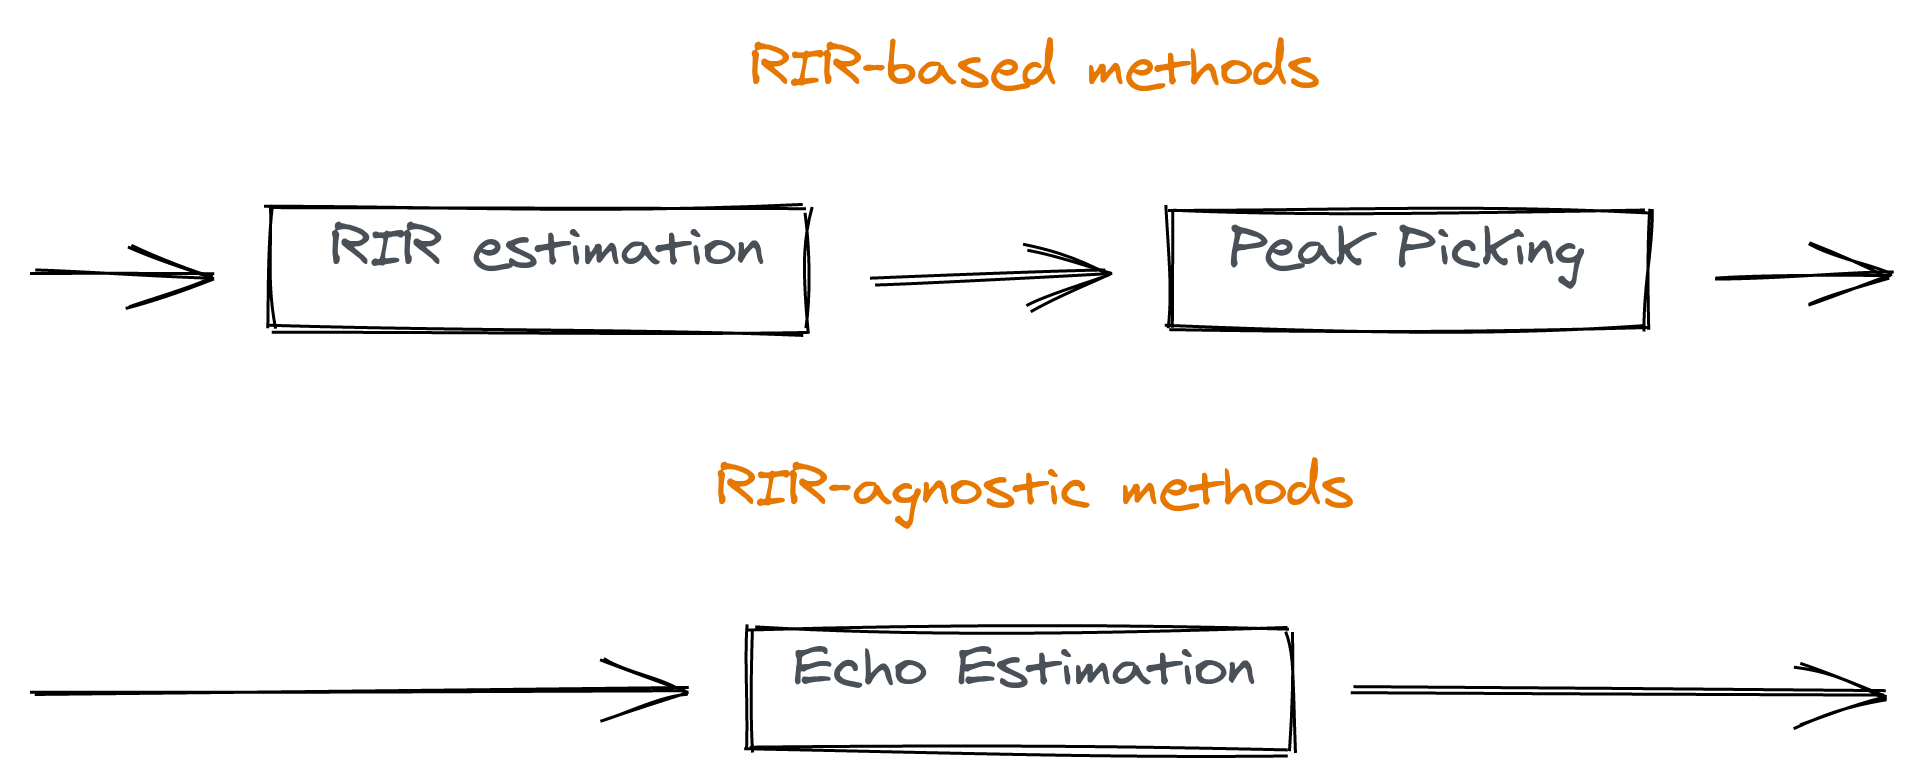
\includegraphics[width=302.12pt,height=122.55pt]{estimation/ch4_estimation_rirbased_agnostic.png}};

% Text Node
\draw (294,89.4) node [anchor=north west][inner sep=0.75pt]  [font=\footnotesize]  {$\tilde{h}_{i}( t)$};
% Text Node
\draw (111,90.9) node [anchor=north west][inner sep=0.75pt]  [font=\footnotesize]  {$\tilde{x}_{i}( t)$};
% Text Node
\draw (111,179.4) node [anchor=north west][inner sep=0.75pt]  [font=\footnotesize]  {$\tilde{x}_{i}( t)$};
% Text Node
\draw (504,92.4) node [anchor=north west][inner sep=0.75pt]  [font=\footnotesize]  {$\left\{\tau ^{( r)}_{i} ,\alpha ^{( r)}_{i}\right\}_{r}$};
% Text Node
\draw (504,182.4) node [anchor=north west][inner sep=0.75pt]  [font=\footnotesize]  {$\left\{\tau ^{( r)}_{i} ,\alpha ^{( r)}_{i}\right\}_{r}$};


\end{tikzpicture}

    }
    \sideparmargin{outer}
    \sidepar{\vspace{-5\baselineskip}
        \captionof{figure}{%
            \footnotesize
            Schematic of \RIR/-based and \RIR/-agnostic approaches.
            }
        \label{fig:estimation:rirbasedagnostic}
    }
    \vspace{-\baselineskip}\vspace{-\baselineskip}
\end{figure}

\mynewline
Given the above categories, we can now review the \AER/ methods presented in the literature.

\section{Literature review}\label{sec:estimation:sota}

\subsection{Active and RIR-based method}\label{subsec:estimation:active_rir}
% In this categories fall all the methods that first attempt for a ``good'' estimation of \RIRs/ for which the reference signal is known.
% The echoes are identified and peaks in the estimated \RIRs/ and ad-hoc techniques are used to identify them.

\newthought{The \RIR/ estimation step} is typically modeled as a deconvolution problem whose performance depends on the type of transmitted signal.
When the transmitted signal can be chosen, several methods were developed to measure real \RIRs/.
Since the \RIR/ corresponds to the room response to a perfect impulse, one can measure it by producing an impulse sound, \eg/ a clap, piercing a balloon, or a gun shot.
Even though these methods are commonly used, they show clear limitations in terms of reproducibility and safety.
Instead, modern computational techniques are used, involving the computation of a deconvolution or \textit{cross-correlation}\sidenote{%
    Cross-correlation and convolution operations are very similar, an mathematically they differ just by the inversion of the reference signal.
    While, the former measures the similarity between two signals as function of a translation, the latter measure the effect of one signal on the other signal.
    See~\cref{subsec:estimation:active_agnostic} for further explanation.
} between the known emitted signal and the recorded output.
The \MLSdef/ technique was first proposed in~\citeonly{schroeder1979integrated} and it is based on the excitation of the acoustical space by a periodic pseudo-random signal, called \MLS/.
The RIR is then calculated by circular correlation between the measured output and the original \MLS/ signal.
This method was further improved in order to achieve better \RIR/ estimation in~\citeonly{aoshima1981computer,dunn1993distortion}.
Unfortunately this technique introduces several artifacts which yield spurious peaks in the estimation.
Moreover, it is sensible to harmonic distortions generally introduced by playback devices, \eg/, the loudspeakers.
\\To overcome these issues, the \ESSdef/ technique was introduced by Farina~\citeonly{farina2000simultaneous,farina2007advancements}.
The probe signal is the \ESS/ signal, \aka/ \textit{chirp signal}, which enjoys the following properties:
the signal spans a user-defined frequency range; it compresses into a narrow impulse during autocorrelation\sidenote{
    Ideally, in an infinite range of frequencies is used, the it compress into a ideal Dirac function.
}; and its Fourier inverse is available in closed form.
The reader can find a review of the presented techniques applied to \RIR/ measurements in~\citeonly{szoke2019building}.
\\Sometimes the reference signal is known, but none of the above techniques can be used.
For instance, when the source signal is narrowband or when the acoustic conditions are challenging.
Therefore the \RIR/ estimation problem needs to be addressed as a more general deconvolution problem, typically solved through optimization methods.
This approach has been well studied in the literature and can be solved using standard Linear Least Squares Error methods with closed-form solutions~\citeonly{krim1996two,glentis1999efficient}
However, in the case of signals with sparse frequency content (\eg/ speech or music) or low SNR, it becomes ill-conditioned and prior knowledge about the \RIR/ is used to improve the estimation, as it will discussed later.

\newthought{Echo Retrieval from RIR.}
As discussed in~\cref{pt:background}, acoustic echoes can be identified as peaks in the early part of the \RIR/.
In general, due to the measurement process, such peaks are not necessarily positive.
Thus, to better visualize them, the \textit{echogram}~\citeonly{kuttruff2016room}, $\magnitudeOf{\tilde{\rir}(t)}$, or the energy envelope\sidenote{
    The energy envelope of a signal is computed as the magnitude of its analytic representation, computed with the Hilbert transform.
    For the signal $x$, its envelope is computed as
    \begin{equation}\label{eq:estimation:hilbert}
        e[n] =  \sqrt{x^2[n] + \calH\kbrace{x}^2[n]}
        ,
    \end{equation}
    where $\calH\kbrace{\cdot}$ denotes Hilbert transform.
}~\citeonly{schroeder1979integrated} are used instead.
\\Provided a good estimation of the \RIRs/, the echoes' locations and amplitudes could be extracted manually by experts.
However, even in an ideal scenario, the automation of this process and the correct identification of such quantities are not straightforward tasks.
As showed in \citeonly{tukuljac2018mulan}, since the \TOAs/ are not necessarily multiples of the sampling grid, their true locations (and amplitudes) are blurred by spurious side peaks.
This issue is referred to as \textit{basis mismatch} in the \textit{compressed sensing} literature.
Although it can be alleviated by increasing the sampling frequency, it is bound to occur in practice.
Moreover, the harmonic distortion due to the non-ideal source-receiver coupling may introduce other spurious peaks as well.
% and reveals the strong limitation of simple \RIR/ peak-pinking.
Furthermore, as noticed in~\citeonly{defrance2008finding}, even small errors in echo' timing estimation may lead to significant differences for echo-based applications.
\\Existing methods for extracting echoes from \RIRs/ can be further dichotomized into two broad categories: \textit{on-grid} and \textit{off-grid} approaches.
The methods belonging to the former group are the most used in practice, and advanced technique are used to cope with the presence of spurious peaks~\citeonly{kuster2008reliability, crocco2017uncalibrated, remaggi2016acoustic, defrance2008detecting, bello2005tutorial, cheng2016attack, defrance2008detecting, annibale2012geometric, kelly2014detecting, usher2010improved}.
\\The most straightforward approach is to deploy iterative and adaptive thresholding algorithms on the \RIR/, followed by robust and manually-tuned peak finders~\citeonly{kuster2008reliability, crocco2017uncalibrated}.
To better inform the peak-picking, several strategies have been proposed.
In the work of~\citeonly{remaggi2016acoustic}, based on a algorithm presented in~\citeonly{naylor2006estimation}, peaks are clustered according to changes in the phase slope of the \RIR/ spectrum.
Other works apply onset detection techniques used in music information retrieval based on edge-detection wavelet filters~\citeonly{bello2005tutorial}, non-negative matrix factorization~\citeonly{cheng2016attack}, or considering the \RIR/'s Kurtosis~\citeonly{usher2010improved}.
\\By noticing that the reflections in the \RIRs/ exhibit a similar shape to the direct path, the author of~\citeonly{defrance2008detecting} first proposed the use of \textit{Matching Pursuit} (and improvements) to identify such shapes.
Here, the direct sound part was used as a pattern (or atom) to be retrieved across the \RIR/.
Unfortunately, in its pure form, this approach is unsuitable for real \RIRs/ because of the frequency-dependent characteristic of the room absorption material.
In order to improve the detection, in~\citeonly{kelly2014detecting} this approach is extended to \textit{Dynamic Time Warping} to account for the non-uniform compression, dilation and concurrency of echoes.
Nevertheless, the idea of exploiting the direct path component to isolate the source-receiver coupling and thus identify first prominent reflections through deconvolution was used in~\citeonly{annibale2012geometric}.
This technique is also referred to as \textit{matching filter} or \textit{direct-path compensation}.
\\Alternative approaches detect the echo timings in another transformed domain.
In \citeonly{vesa2010segmentation} the echoes are localized in the \TFdef/ domain using cross-wavelet transform based on previous works~\citeonly{guillemain1996characterization, loutridis2005decomposition}.
In \citeonly{peled2013linearly}, the authors propose to identify the direction of arrival of the reflections in the spherical harmonic domain using plane wave decomposition.
The works~\citeonly{ristic2013detection,pavlovic2016multifractal} use (multi-)fractal analysis to detect echoes in the \TFdef/ domain.
Alternatively, the authors of~\citeonly{ferguson2019improved,jia2017extraction} propose to identify echoes properties in the cepstral domain.
The \textit{cepstrum} is usually defined as the inverse Fourier transform of the logarithmic magnitude spectrum.\sidenote{
    There are several concurrent definitions of cepsturm. For a given time-domain signal $\tildex$ it is usually defined as
    $\powerOf{\fourierTrans^{-1}\kbrace{\log{\powerOf{\fourierTrans{x}}}}}$, where $\fourierTrans$ is the \FT/ operator.
} One interesting property of the cepstrum is to separate the spectral envelop form the line-spectra components in different ``quefrency'' ranges.
Therefore, it is used to detect periodicity in the spectrum of the observed signal, with many applications in speech processing as well as in hydraulic and mechanic applications.
This approach seems promising since time-domain peaks are mapped to complex sinusoids in the frequency domain.
However, this representation is highly sensible to external and sampling noise and the accuracy is limited by the approximation of the \DFT/ operator.

\mynewline
All the above mentioned active and \RIR/-based works aim at detecting echoes on the sampling grid.
In order to face the inherent limitations of these approaches, off-grid frameworks have been proposed, \eg/~\citeonly{condat2013robust}.
This approach can be related to classical \MLdef/ estimation approaches, which consist in selecting the model which is most likely to explain the observed noisy data.
In this category fall classical spectral estimation techniques, \eg/ \MUSIC/~\citeonly{loutridis2005decomposition}, \ESPRIT/~\citeonly{roy1986esprit}, which are fast but statistically suboptimal.
The method presented in \citeonly{condat2013robust} focuses on the general problem of estimating a finite stream of Dirac's impulses from uniform, noisy and lowpass-filtered samples.
The authors showed that this particular problem can be reformulated as \textit{matrix denoising}, from which the echoes' locations and amplitudes can be retrieved in closed-form.
Although this method reaches the statistical optimality in the \ML/ sense, the exact knowledge of the number of Diracs needs to be known in advance.
If this number is unknown or approximated, errors in the estimation are observed.
This results in a drawback since the exact number of echoes is difficult to know a priori and false-positive peaks are present even in clean \RIRs/ due to the source's harmonic distortions or limited bandwidth.

\mynewline
That being said, \AER/ is far from trivial even when clean \RIR/ estimates are provided.
It is important to note that, for every \TOA/ estimator, a practical trade off exists between the number of missed \TOAs/ (false negative) and the number of spurious \TOAs/ (false positive).
This trade-off is only partially dependent on the noise level since many factors can provide spurious peaks.
For instance, side lobes due to finite signal bandwidth, echo distortions due to frequency dependent attenuations and coalescing peaks due to close \TOAs/ can affect peak estimation.
This fact is often a source of unavoidable outliers that make the robustness of subsequent steps in echo-aware applications a delicate and very important issue.
A way to overcome this trade-off is to allows spurious \TOAs/ estimates and prune them using echo labeling afterwards.

\newthought{Echo Labeling or \TOAs/ Disambiguation} \marginpar{
    \footnotesize
    \centering
    \resizebox{\linewidth}{!}{
        

\tikzset{every picture/.style={line width=0.75pt}} %set default line width to 0.75pt

\begin{tikzpicture}[x=0.75pt,y=0.75pt,yscale=-1,xscale=1]
%uncomment if require: \path (0,300); %set diagram left start at 0, and has height of 300

%Shape: Rectangle [id:dp14567992755438064]
\draw  [draw opacity=0][fill={rgb, 255:red, 255; green, 255; blue, 255 }  ,fill opacity=1 ] (120,150) -- (140,150) -- (140,170) -- (120,170) -- cycle ;
%Image [id:dp10534507113138725]
\draw (130,160) node  {
\includegraphics[width=15pt,height=15pt]{figures/acoustics/iconfinder_ic_speaker_48px_352138.pdf}};

%Straight Lines [id:da5739497937229707]
\draw [color={rgb, 255:red, 245; green, 166; blue, 35 }  ,draw opacity=1 ]   (140,150) -- (150,80) -- (158.66,97.32) ;
\draw [shift={(160,100)}, rotate = 243.43] [fill={rgb, 255:red, 245; green, 166; blue, 35 }  ,fill opacity=1 ][line width=0.08]  [draw opacity=0] (5.36,-2.57) -- (0,0) -- (5.36,2.57) -- cycle    ;
%Straight Lines [id:da8578730942455487]
\draw [color={rgb, 255:red, 245; green, 166; blue, 35 }  ,draw opacity=1 ]   (140,150) -- (180,80) -- (208.2,117.6) ;
\draw [shift={(210,120)}, rotate = 233.13] [fill={rgb, 255:red, 245; green, 166; blue, 35 }  ,fill opacity=1 ][line width=0.08]  [draw opacity=0] (5.36,-2.57) -- (0,0) -- (5.36,2.57) -- cycle    ;
%Shape: Rectangle [id:dp5076369836155045]
\draw   (240,80) -- (110,80) -- (110,180) -- (240,180) -- cycle ;
%Straight Lines [id:da22242030089201148]
\draw [color={rgb, 255:red, 155; green, 155; blue, 155 }  ,draw opacity=1 ]   (140,150) -- (240,140) -- (222.68,131.34) ;
\draw [shift={(220,130)}, rotate = 386.57] [fill={rgb, 255:red, 155; green, 155; blue, 155 }  ,fill opacity=1 ][line width=0.08]  [draw opacity=0] (5.36,-2.57) -- (0,0) -- (5.36,2.57) -- cycle    ;
%Image [id:dp1558986620539785]
\draw (165,105) node  {
\includegraphics[width=7.5pt]{figures/acoustics/iconfinder_microphone_1608550.pdf}};
%Straight Lines [id:da8481877472892685]
\draw [color={rgb, 255:red, 155; green, 155; blue, 155 }  ,draw opacity=1 ]   (140,150) -- (240,130) -- (172.88,110.82) ;
\draw [shift={(170,110)}, rotate = 375.95] [fill={rgb, 255:red, 155; green, 155; blue, 155 }  ,fill opacity=1 ][line width=0.08]  [draw opacity=0] (5.36,-2.57) -- (0,0) -- (5.36,2.57) -- cycle    ;
%Image [id:dp09126870353707106]
\draw (215,125) node  {
\includegraphics[width=7.5pt]{figures/acoustics/iconfinder_microphone_1608550.pdf}};
%Straight Lines [id:da3123556849021565]
\draw [color={rgb, 255:red, 245; green, 166; blue, 35 }  ,draw opacity=1 ]   (280,120) -- (280,90.34) ;
\draw [shift={(280,90)}, rotate = 270] [color={rgb, 255:red, 245; green, 166; blue, 35 }  ,draw opacity=1 ][line width=0.75]      (0, 0) circle [x radius= 1.34, y radius= 1.34]   ;
%Straight Lines [id:da13538016730145752]
\draw [color={rgb, 255:red, 155; green, 155; blue, 155 }  ,draw opacity=1 ]   (300,120) -- (300,100.34) ;
\draw [shift={(300,100)}, rotate = 270] [color={rgb, 255:red, 155; green, 155; blue, 155 }  ,draw opacity=1 ][line width=0.75]      (0, 0) circle [x radius= 1.34, y radius= 1.34]   ;
%Straight Lines [id:da7530423918162308]
\draw [color={rgb, 255:red, 245; green, 166; blue, 35 }  ,draw opacity=1 ]   (296,180) -- (296,160.34) ;
\draw [shift={(296,160)}, rotate = 270] [color={rgb, 255:red, 245; green, 166; blue, 35 }  ,draw opacity=1 ][line width=0.75]      (0, 0) circle [x radius= 1.34, y radius= 1.34]   ;
%Straight Lines [id:da29932347303901585]
\draw [color={rgb, 255:red, 155; green, 155; blue, 155 }  ,draw opacity=1 ]   (287,180) -- (287,150.34) ;
\draw [shift={(287,150)}, rotate = 270] [color={rgb, 255:red, 155; green, 155; blue, 155 }  ,draw opacity=1 ][line width=0.75]      (0, 0) circle [x radius= 1.34, y radius= 1.34]   ;
%Straight Lines [id:da7781666726084306]
\draw    (260,120) -- (260,83) ;
\draw [shift={(260,80)}, rotate = 450] [fill={rgb, 255:red, 0; green, 0; blue, 0 }  ][line width=0.08]  [draw opacity=0] (3.57,-1.72) -- (0,0) -- (3.57,1.72) -- cycle    ;
%Straight Lines [id:da1325246921812081]
\draw    (260,120) -- (327,120) ;
\draw [shift={(330,120)}, rotate = 180] [fill={rgb, 255:red, 0; green, 0; blue, 0 }  ][line width=0.08]  [draw opacity=0] (3.57,-1.72) -- (0,0) -- (3.57,1.72) -- cycle    ;
%Straight Lines [id:da5562759989146545]
\draw    (260,180) -- (260,143) ;
\draw [shift={(260,140)}, rotate = 450] [fill={rgb, 255:red, 0; green, 0; blue, 0 }  ][line width=0.08]  [draw opacity=0] (3.57,-1.72) -- (0,0) -- (3.57,1.72) -- cycle    ;
%Straight Lines [id:da49505321657128565]
\draw    (260,180) -- (327,180) ;
\draw [shift={(330,180)}, rotate = 180] [fill={rgb, 255:red, 0; green, 0; blue, 0 }  ][line width=0.08]  [draw opacity=0] (3.57,-1.72) -- (0,0) -- (3.57,1.72) -- cycle    ;

% Text Node
\draw (119,82) node [anchor=north west][inner sep=0.75pt]  [font=\tiny] [align=left] {wall $\displaystyle i$};
% Text Node
\draw (238,151) node [anchor=north west][inner sep=0.75pt]  [font=\tiny,rotate=-90] [align=left] {wall $\displaystyle j$};
% Text Node
\draw (117,162.4) node [anchor=north west][inner sep=0.75pt]  [font=\tiny]  {$\positionSource$};
% Text Node
\draw (157,115.4) node [anchor=north west][inner sep=0.75pt]  [font=\tiny]  {$\positionMicrophone_{1}$};
% Text Node
\draw (207,135.4) node [anchor=north west][inner sep=0.75pt]  [font=\tiny]  {$\positionMicrophone_{2}$};
% Text Node
\draw (312,132) node [anchor=north west][inner sep=0.75pt]  [font=\tiny] [align=left] {time};
% Text Node
\draw (312,182) node [anchor=north west][inner sep=0.75pt]  [font=\tiny] [align=left] {time};
% Text Node
\draw (261,132.4) node [anchor=north west][inner sep=0.75pt]  [font=\tiny]  {$\tildex_{2}$};
% Text Node
\draw (261,72.4) node [anchor=north west][inner sep=0.75pt]  [font=\tiny]  {$\tildex_{1}$};
% Text Node
\draw (282,87.4) node [anchor=north west][inner sep=0.75pt]  [font=\tiny]  {$i$};
% Text Node
\draw (302,97.4) node [anchor=north west][inner sep=0.75pt]  [font=\tiny]  {$j$};
% Text Node
\draw (298,156.4) node [anchor=north west][inner sep=0.75pt]  [font=\tiny]  {$i$};
% Text Node
\draw (288,146.4) node [anchor=north west][inner sep=0.75pt]  [font=\tiny]  {$j$};


\end{tikzpicture}

    }
    \captionof{figure}{Illustration of different orders of arrival of wall reflections}
    \label{fig:estimation:labeling}
} is the task of assigning acoustic echoes to different image sources or reflectors, as shown in~\cref{fig:estimation:labeling}.
Many methods have been proposed in the context of \SSL/~\citeonly{scheuing2006disambiguation, zannini2010improved}, microphone calibration~\citeonly{parhizkar2014single,salvati2016sound}
and \RooGE/~\citeonly{antonacci2010geometric, filos2011robust, venkateswaran2012localizing, antonacci2012inference, dokmanic2013acoustic, crocco2014towards, jager2016room, el2017time}.
A brief review of these methods is provided in~\citeonly{crocco2017uncalibrated}.
\\In the context of \SSL/, the disambiguation is typically performed in the \TDOA/ space~\citeonly{scheuing2006disambiguation, zannini2010improved}.
Moreover these works focus on actively localizing (the direction of arrival of) multiple sources while discarding reflections, rather than localizing the actual image sources.
\\Other disambiguation schemes are typically used for \RooGE/.
In \citeonly{venkateswaran2012localizing} the pruning of the combinatorial candidate-image-source search is done through Bayesian inference.
A similar approach can be found in~\citeonly{dokmanic2013acoustic, parhizkar2014single} where the validity check is based on a particular structured matrix called \textit{Euclidean Distance Matrix} and further improved using compatibility graphs in~\citeonly{jager2016room}.
These methods rely on a combinatorial search with a potentially high number of candidates, which leads to intractable computational complexity when multiple reflections are considered.
Moreover these methods require that all the distances between microphones are known with precision, which may not be true in practice.
\\In the works of~\citeonly{antonacci2010geometric, filos2011robust, antonacci2012inference}, the reflectors are modelled as planes tangent to ellipsoids with foci given by each pair of microphone/source, as shown in~\cref{fig:estimation:ellips}.\marginpar{
    \footnotesize
    \centering
    \resizebox{\linewidth}{!}{
        

\tikzset{every picture/.style={line width=0.75pt}} %set default line width to 0.75pt

\begin{tikzpicture}[x=0.75pt,y=0.75pt,yscale=-1,xscale=1]
%uncomment if require: \path (0,300); %set diagram left start at 0, and has height of 300

%Shape: Rectangle [id:dp966627560130513]
\draw  [draw opacity=0][fill={rgb, 255:red, 255; green, 255; blue, 255 }  ,fill opacity=1 ] (70.8,159.6) -- (105.2,159.6) -- (105.2,193.6) -- (70.8,193.6) -- cycle ;
%Image [id:dp3167807043537194]
\draw (88,176.6) node  {
\includegraphics[width=25.8pt,height=25.5pt]{figures/acoustics/iconfinder_ic_speaker_48px_352138.pdf}};

%Shape: Rectangle [id:dp36313703479455617]
\draw  [draw opacity=0][fill={rgb, 255:red, 155; green, 155; blue, 155 }  ,fill opacity=1 ] (225.11,90) -- (210,90) -- (210,240) -- (225.11,240) -- cycle ;
%Straight Lines [id:da052649281163546946]
\draw    (210,90) -- (210,240) ;
%Straight Lines [id:da4220394126624911]
\draw [color={rgb, 255:red, 245; green, 166; blue, 35 }  ,draw opacity=1 ] [dash pattern={on 4.5pt off 4.5pt}]  (88,181) -- (210.26,154.35) ;
\draw [shift={(88,181)}, rotate = 347.7] [color={rgb, 255:red, 245; green, 166; blue, 35 }  ,draw opacity=1 ][fill={rgb, 255:red, 245; green, 166; blue, 35 }  ,fill opacity=1 ][line width=0.75]      (0, 0) circle [x radius= 2.34, y radius= 2.34]   ;
%Shape: Rectangle [id:dp9150839162633834]
\draw  [draw opacity=0][fill={rgb, 255:red, 255; green, 255; blue, 255 }  ,fill opacity=1 ] (311.6,160) -- (346,160) -- (346,194) -- (311.6,194) -- cycle ;
%Image [id:dp4871405033106181]
\draw (328.8,177) node  {
\includegraphics[width=25.8pt,height=25.5pt]{figures/acoustics/iconfinder_ic_speaker_48px_352138.pdf}};

%Shape: Rectangle [id:dp8153393136177459]
\draw  [draw opacity=0][fill={rgb, 255:red, 255; green, 255; blue, 255 }  ,fill opacity=0.45 ] (312.9,157.09) -- (342.23,157.09) -- (342.23,194.47) -- (312.9,194.47) -- cycle ;
%Straight Lines [id:da7529808549768326]
\draw  [dash pattern={on 4.5pt off 4.5pt}]  (208,154) -- (328.85,182.59) ;
\draw [shift={(328.85,182.59)}, rotate = 13.31] [color={rgb, 255:red, 0; green, 0; blue, 0 }  ][fill={rgb, 255:red, 0; green, 0; blue, 0 }  ][line width=0.75]      (0, 0) circle [x radius= 2.34, y radius= 2.34]   ;
%Shape: Ellipse [id:dp26881919866041726]
\draw  [color={rgb, 255:red, 245; green, 166; blue, 35 }  ,draw opacity=1 ][dash pattern={on 0.84pt off 2.51pt}] (63.3,192.06) .. controls (51.39,161.77) and (73.54,124.71) .. (112.77,109.28) .. controls (152,93.85) and (193.45,105.9) .. (205.37,136.19) .. controls (217.28,166.47) and (195.13,203.53) .. (155.9,218.96) .. controls (116.67,234.39) and (75.21,222.35) .. (63.3,192.06) -- cycle ;
%Image [id:dp7990623154835439]
\draw (168,145.5) node  {
\includegraphics[width=12.9pt]{figures/acoustics/iconfinder_microphone_1608550.pdf}};
%Straight Lines [id:da4297672152509986]
\draw [color={rgb, 255:red, 245; green, 166; blue, 35 }  ,draw opacity=1 ] [dash pattern={on 4.5pt off 4.5pt}]  (180.05,145.79) -- (210.26,154.35) ;
\draw [shift={(210.26,154.35)}, rotate = 15.82] [color={rgb, 255:red, 245; green, 166; blue, 35 }  ,draw opacity=1 ][fill={rgb, 255:red, 245; green, 166; blue, 35 }  ,fill opacity=1 ][line width=0.75]      (0, 0) circle [x radius= 2.34, y radius= 2.34]   ;
\draw [shift={(180.05,145.79)}, rotate = 15.82] [color={rgb, 255:red, 245; green, 166; blue, 35 }  ,draw opacity=1 ][fill={rgb, 255:red, 245; green, 166; blue, 35 }  ,fill opacity=1 ][line width=0.75]      (0, 0) circle [x radius= 2.34, y radius= 2.34]   ;

% Text Node
\draw (188.78,91.8) node [anchor=north west][inner sep=0.75pt]  [font=\tiny] [align=left] {wall $\displaystyle i$};
% Text Node
\draw (101.16,192.85) node [anchor=north west][inner sep=0.75pt]  [font=\tiny]  {$\positionSource$};
% Text Node
\draw (153.84,146.3) node [anchor=north west][inner sep=0.75pt]  [font=\tiny]  {$\positionMicrophone$};
% Text Node
\draw (299.56,191.65) node [anchor=north west][inner sep=0.75pt]  [font=\tiny]  {$\mathring{\positionSource}$};

\draw   (143.8, 176.37) circle [x radius= 5, y radius= 5]   ;
\draw   (126.6, 175.02) circle [x radius= 5, y radius= 5]   ;
\draw   (178.2, 195) circle [x radius= 5, y radius= 5]   ;
\draw   (147.91, 212.96) circle [x radius= 5, y radius= 5]   ;
\draw   (178.2, 195) circle [x radius= 5, y radius= 5]   ;
\draw   (152.02, 177.87) circle [x radius= 5, y radius= 5]   ;
\draw   (178.2, 195) circle [x radius= 5, y radius= 5]   ;
\end{tikzpicture}

    }
    \captionof{figure}{Illustration of the ellipsoid method: the length of the reflected path from the image source $\mathring{\positionSource}$ to the microphone at $\positionMicrophone$ constrain the reflector line to
    be tangent to an ellipse.}
    \label{fig:estimation:ellips}
} By solving a non-convex optimization problem based on geometrical reasoning and the Hough transform\sidenote{%
    A mathematical operator that maps points into curves in a 2-D space.
    If a set of points belongs to the same line, the corresponding curves will intersect in a single point.
    In computer vision, this tranform is typically used as feature extractor to detect lines and edges in pictures.
}, they are able to disambiguate \TOAs/ and reconstruct the reflectors' positions and orientations.
However, they all require a very specific acquisition setup and the optimized non-convex cost functions are sensible to local minima.

\mynewline
In general, none of the above methods come with specific strategies to cope with missing or spurious echo estimates.
These may be due to malfunctioning of the peak finder or by erroneous selection of peaks corresponding to higher reflection order.
A way to solve this issue is to exploit particular prior knowledge.
For instance, the approach presented in~\citeonly{el2017time} exploits the shapes of linear and compact arrays of loudspeakers, which provides a natural ordering among the loudspeakers.
By stacking side-by-side the measured \RIRs/ in a matrix, they can be visualized as an image.
Here the wavefront of each reflection draws specific patterns which can be identified easily and robustly even in the presence of (a few) spurious and missing peaks.
Moreover, this approach avoids the combinatorial search.
However, it requires a very specific setup for recordings.
\\In the work~\citeonly{crocco2014towards} an iterative strategy is used.
First, the direct path arrivals are used to estimate a first guess of the microphones and source positions.
Then, the whole set of extracted peaks are used to estimate the planar reflectors' positions which are then used to refine the microphones and source localization.
Alternating between the geometrical space of microphones and source coordinates and the signal space of the echoes' \TOAs/, the ambiguous peaks are pruned during the optimization.

\subsection{Active and RIR-agnostic method}\label{subsec:estimation:active_agnostic}
This class of methods uses the signal at the microphones to directly estimate the echoes reflections, rather than estimating the \RIRs/.
Here two different approaches can be identified: optimization-based approaches~\citeonly{jensen2019method, saqib2020estimation} and cross-correlation-based approaches~\citeonly{crocco2014towards, al2019early}.

\mynewline
The former approaches exploit the strong relation between the \ac{TOA} of an echo with its \ac{DOA}.
When multiple microphones are used and their geometry is known, the relation between these two quantities can be express in closed-form and used in an \ML/-based frameworks.
By modeling the \ac{DOA}s, such approaches are able to implicitly reduce the ambiguity of the estimated echoes.
This idea is rooted in existing methods used in multipath communication systems, denoted as \ac{JADE}~\citeonly{vanderveen1997joint,verhaevert2004direction}.

\mynewline
Alternatively, the echo contributions can be extracted from the \textit{cross-correlation} between the observed and the reference signals.
Cross-correlation analysis is a mathematical tool for the identification of repeated patterns in a signal as a function of a certain time lag.
Due to indoor sound propagation, the received signal consists in repeated copies of the emitted signal.
Therefore, the received signal may correlate with the emitted one for certain time lags.
Hence, peaks in the cross-correlation function can be observed.
By the extraction of these peaks, echoes' \TOAs/ and relative amplitudes can be identified.
This approach was used in \citeonly{tervo2011estimation, crocco2014towards, al2019early}.

When the array geometry is known, the time lag axes of cross-correlation functions between channels can be mapped to possible 2D directions of arrivals (elevation and azimuth), namely from \TOAs/ to 2D-\DOAs/.
The identification of strong reflections can then be performed in the so-called \textit{angular spectrum} domain~\citeonly{dibiase2001robust}.
With a proper clustering approach, the reflections can be inspected, disambiguated and their \TOAs/ deduced.
This approach is used in~\citeonly{o2008imaging, o2010automatic, tervo2015direction} and can be generalized by spatial filtering methods, such as steered-response power-based beamforming.
In~\citeonly{o2008imaging}, it was referred to as \textit{acoustic camera} since it benefits from the following visual interpretation:
as shown in~\cref{fig:estimation:audiocamera}, the 2D-polar Coordinates can be mapped into cartesian ones so that the angular spectrum can be superimposed to a panoramic picture of the audio scene taken by the barycenter of the recording arrays.
\marginpar{
    \centering
    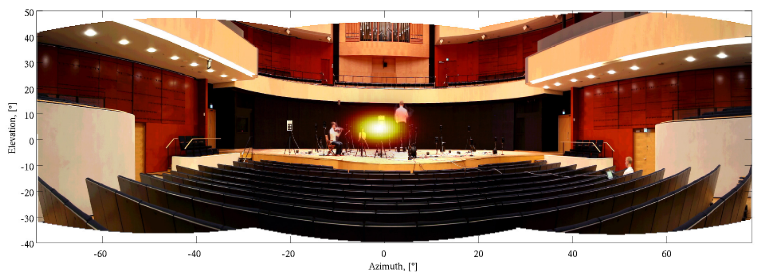
\includegraphics[width=\linewidth]{estimation/audio_camera1.png}
    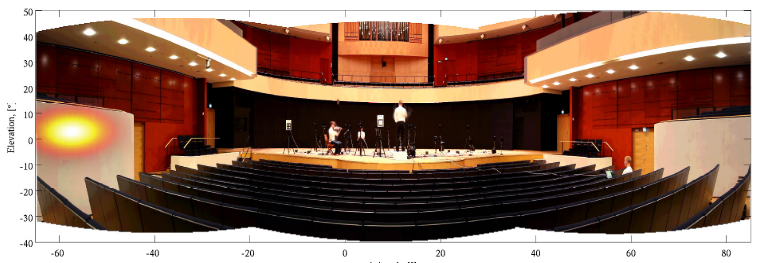
\includegraphics[width=\linewidth]{estimation/audio_camera2.png}
    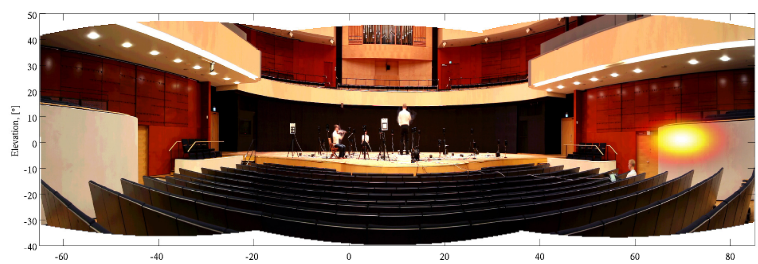
\includegraphics[width=\linewidth]{estimation/audio_camera3.png}
    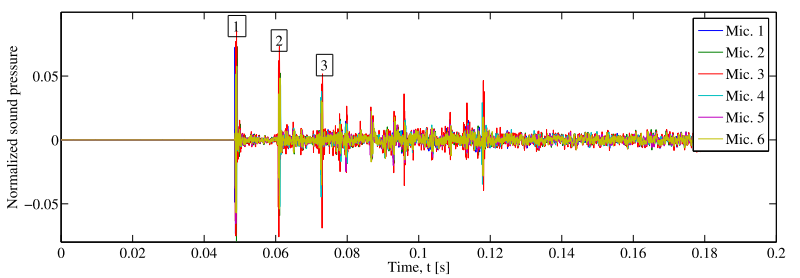
\includegraphics[width=\linewidth]{estimation/audio_camera4.png}
    \captionof{figure}{
        \footnotesize
        Visualization of the \textit{audio camera}:
        The angular spectrum is overlapped to the corresponding images.
        Also shown are the impulse responses for 6 microphones.
        The numbered boxes indicate events shown in the audio camera.
        Images from~\citeonly{tervo2011localization}.}
    \label{fig:estimation:audiocamera}
}

\subsection{Passive and RIR-based method}\label{subsec:estimation:bce}
Passive approaches
\marginpar{
    \footnotesize
    \emph{
    The innovative idea of passive \BCE/ can be traced back to~\citeonly{sato1975method}.
    A review of the the evolution of \SIMO/ \BCE/ can be found in~\citeonly{huang2003class}.
}} rely on external, unknown sound sources in the environment to conduct the estimation.
In the literature, this problem belongs to the broad and deeply studied category of \BCEdef/ or \BSIdef/ problems.
In the particular case of a single source, it is referred to as \SIMO/ \BCE/.
Common to all these methods is the assumption that \RIRs/ are discrete \FIR/ filters defined on the sampling grid, namely, vectors in the Euclidean space.
In the general setting of arbitrary signals and filters, rigorous theoretical ambiguities under which the problem is ill-posed have been identified~\citeonly{xu1995least}.
Some well-known limitations of these approaches are their sensitivity to the chosen length of the filters, and their intractability when the filters are too large.
\FIR/ \SIMO/ \BCE/ can be broadly dichotomized into the class of \textit{statistical methods} and the class of \textit{blind methods}.

\newthought{Statistical methods} exploit knowledge about the emitted signal.
Since the nature of the source signal is often non-deterministic and it statistics can be modeled based on the signal category, \eg/ speech or music.
Two main approaches can be identified~\citeonly{tong1998multichannel}:
\begin{itemize}
    \item \textit{Second Order Moments approaches} derive closed-form solutions for which the knowledge of the source auto-correlation function is required.
    \item \textit{Maximum Likelihood approaches} require instead the source probability function.
    Even though they are optimal in the \ML/ sense, they optimize non-convex cost functions, typically via \EMdef/.
    In this category one may include the methods developed for multichannel blind source separation~\citeonly{ozerov2009multichannel,duong2010under,sawada2013multichannel,leglaive2016multichannel,leglaive2018student,scheibler2018separake}.
    These methods are built on the well-studied framework of Multichannel \NMF/~\citeonly{ozerov2009multichannel,sawada2013multichannel} which lends itself to account for various types of side information.
    Here the source signals are typically modeled as Gaussian distributions centred at zero and with unknown variances.
    In general, they aim at estimating both the acoustic channels and the source contribution.
    In particular, the work of~\citeonly{duong2010under} extends this framework to reverberant recordings using physics-based models for the late reverberation, while the works of~\citeonly{leglaive2016multichannel} considers explicitly the contribution of early echoes, further improved in~\citeonly{leglaive2018student}.
    % It is important to notice, that all the methods listed here
\end{itemize}
Even if statistical methods have reported a considerable success in the field of sound source separation, they play a minor role in \RIR/ estimation.
This is due to the difficulty of estimating reliable statistics of the emitted signals or a good initialization point required by the \EM/ algorithm.
Moreover, although the final estimated \RIRs/ may match the real ones in the statistical sense, they lack a sufficient level of details, indispensable for \AER/.
\marginpar{
    \centering
    \footnotesize
    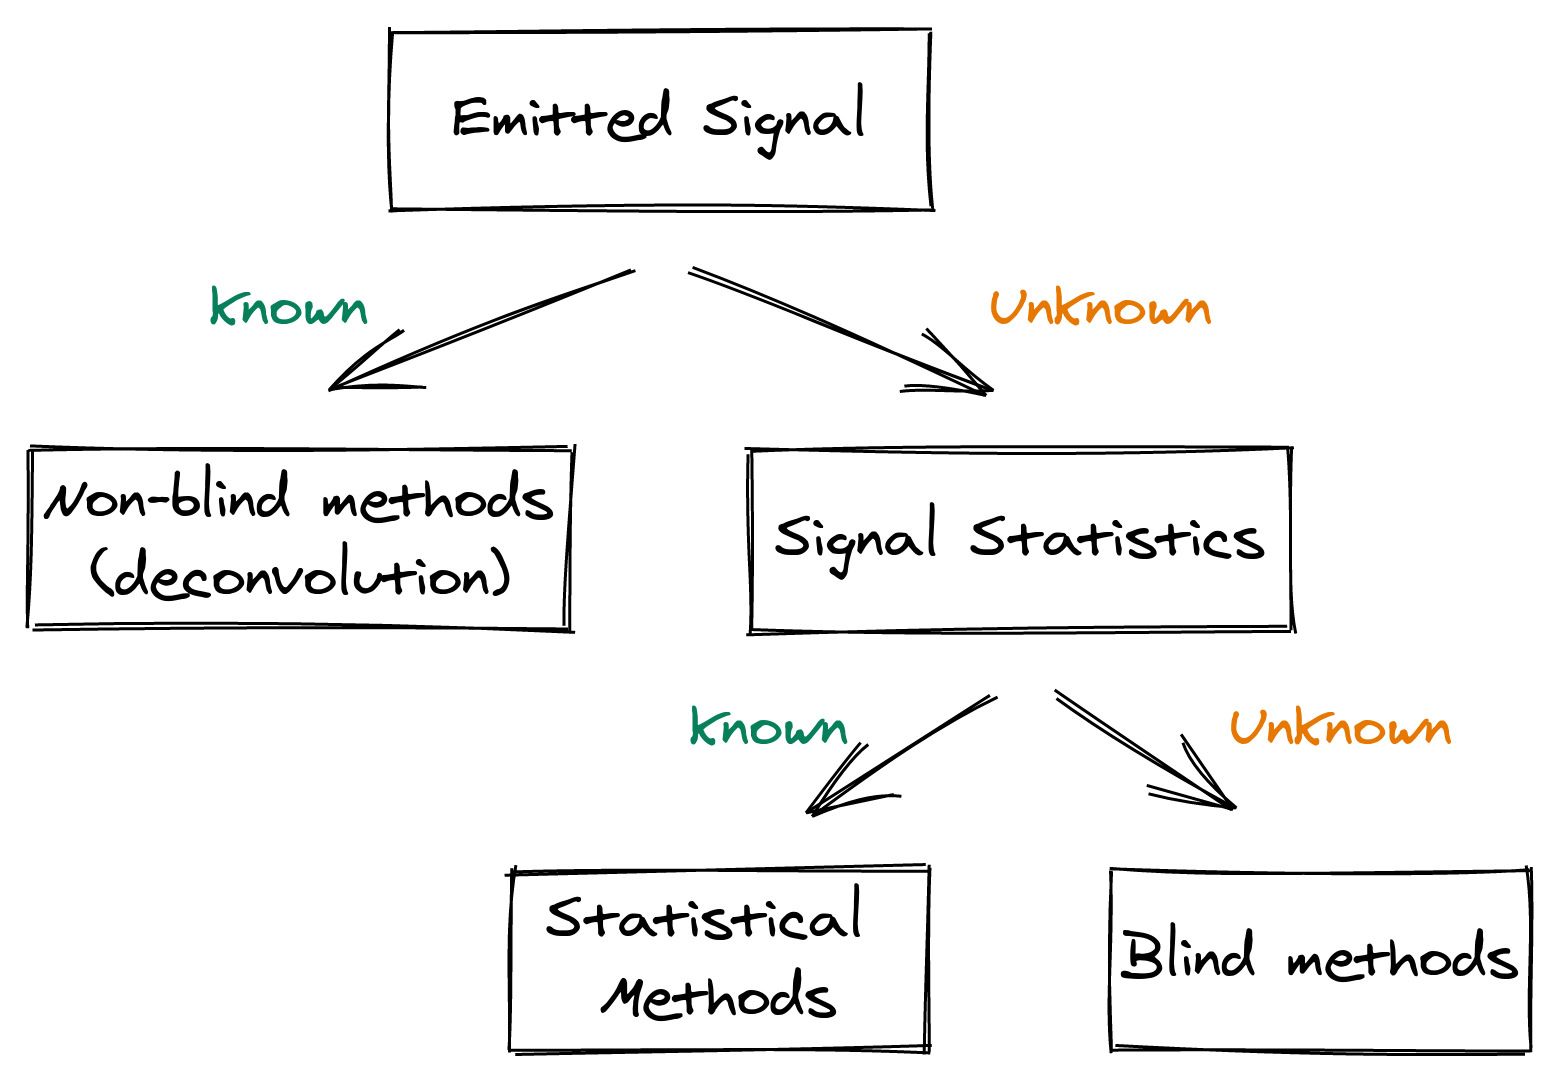
\includegraphics[trim={0 0 0 0},clip,width=\linewidth]{estimation/ch4_estimation_bce_sota.png}
    \captionof{figure}{%
        Classification of the State of the Art in channel estimation.
    }
    \label{fig:estimation:sotabce}
}


\newthought{Blind methods} comprises two main groups: \textit{subspace} methods~\citeonly{abed1997subspace} and \textit{cross-relation methods}~\citeonly{tong1994blind,xu1995least,lin2007blind,lin2008blind,kowalczyk2013blind,crocco2015room,crocco2016estimation}.
The formers are based on the key idea that the channel (or part of it ) vector spans a one-dimensional subspace of noiseless observations.
These methods have the attractive property that the channel estimates can often be obtained in closed-form by optimizing a quadratic cost function.
However that they are typically computationally expensive and sensible to noise.
% However they may not be robust, especially when the channel covariance matrix is close to being singular.
\\The second family of methods rely on the clever observation that in the noiseless case, for every pair of microphone $(i, i')$, it holds that
\begin{equation}\label{eq:estimation:xrel_toepl}
    (\tildex_{i'} \convCont \tildeh_i)(t) = (\tildex_{i} \convCont \tildeh_{i'})(t) =  ((\tildeh_{i'} \convCont \tildeh_i) \convCont s)(t)
    ,
\end{equation}
by commutativity and associativity of the convolution operator.
This identity is called the \textit{cross-relation} and it was first introduced by~\citeonly{tong1994blind}.
In this work, the \RIR/ are estimated by solving a Least Square minimization of the sum of square cross-relation errors.
In \citeonly{xu1995least,tong1998multichannel}, sufficient and necessary conditions for channel identification are discussed.
This approach has received significant attention as it does not require any assumption about the source signal.
Later, the accuracy of estimated \RIRs/ has been subsequently improved using prior knowledge on the filters:
in particular, the authors of~\citeonly{lin2007blind} have proposed to use sparsity penalty and non-negativity constraints to increase robustness to noise as well as Bayesian-learning methods to automatically infer the value of the hyper-parameters in~\citeonly{lin2008blind}.
Even if sparsity and non-negativity could be seen as a strong assumptions, works in speech enhancement~\citeonly{ribeiro2010turning,dokmanic2015raking} and room geometry estimation~\citeonly{antonacci2012inference,crocco2017uncalibrated} have proven the effectiveness of this approach.
On a similar scheme, in~\citeonly{kowalczyk2013blind}, the problem in~\cref{eq:estimation:xrel_toepl} is solved using an adaptive time-frequency-domain approach while~\citeonly{aissa2008blind} proposes to use the $\ell_p$-norm instead of the $\ell_1$-norm.
A successful approach has been presented by Crocco \textit{et al.} in \citeonly{crocco2015room,crocco2016estimation}, where the so-called \textit{anchor constraint} is replaced by an \textit{iterative weighted} $\ell_1$ equality constraint to better balance sparsity penalty and the model constraints.\sidenote{
    These approaches will be further formalized and detailed in~\cref{ch:blaster}.
}
Finally, the very recent work~\citeonly{qi2019broadband} extends cross-relation approaches under the umbrella of the Kalman filter which was previously used for echo-cancellation applications.
\\An alternative approach is used in~\citeonly{cmejla2019mirage}, where the \ReIR/ estimation problem is treated as a special case of \ReIR/ estimation.
As mentioned in~\cref{subsec:processing:rtf}, in the noiseless case, the \ReIR/ identifies to the \ReIR/ when the reference microphone is placed very close to the source.
\ReIR/ estimation found its root in the field of \SEdef/~\citeonly{gannot2001signal} and many techniques have been proposed since then~\citeonly{gannot2001signal,koldovsky2015spatial,koldovsky2015sparse,kodrasi2017evd}.
By its definition, in the noiseless case, the \ReIR/ describes the relative filter between two observations and not directly their \RIRs/.
The main limitation of this approach is that it is possible only in controlled scenarios, where the user has the possibility to place the microphone arbitrarily in the room and in the presence of high \ac{SNR} levels.
Nevertheless, in this context, this particular setup is found to be useful not only for \RTF/ estimation, but also for microphone calibration, since it allows to solve geometrical ambiguities, yielding a closed-form solution, as done in~\citeonly{crocco2012closed}.

\mynewline
In general, the main drawbacks of \FIR/ \SIMO/ \BCE/ works is that they rely on on-grid estimation, sparsity-enforcing regularizers and peak-picking which need to be tuned manually.
As described in~\cref{sec:processing:fouriermodel}, due to the sampling process involving an ideal low-pass kernel, the filters are non-sparse and non-negative.
This general bottleneck has been referred to as \textit{basis mismatch} and was notably studied in the \textit{compressed sensing} community~\citeonly{chi2011sensitivity}.
In particular, the true peaks in the \RIR/ do not necessarily correspond to the true echoes as shown in~\cref{fig:estimation:mismatch}.
\begin{figure}[h]
    \begin{fullwidth}
        \centering
        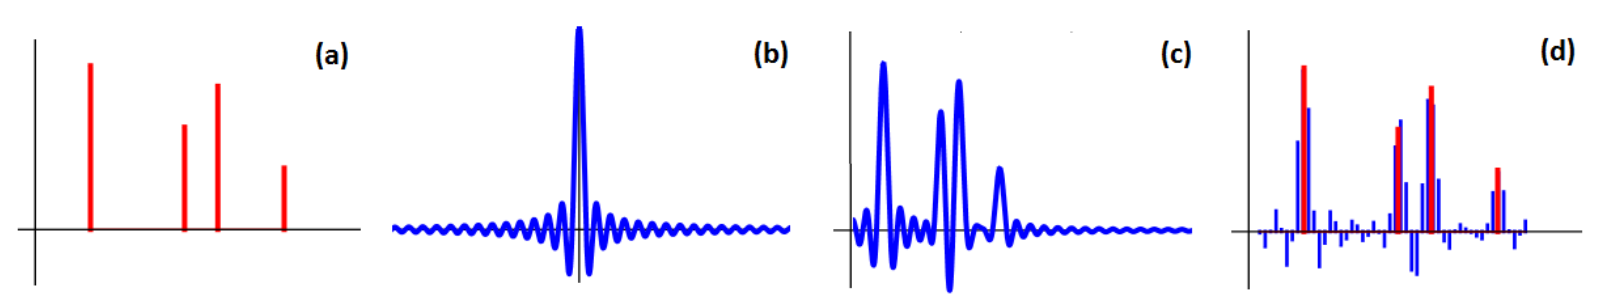
\includegraphics[width=\linewidth]{estimation/basismismatch.png}
        \caption{%
        (a) Continuos-time stream of Diracs $\tilde{h}(t)$,
        (b) sinc kernel $\lowpassfilter(t)$,
        (c) smoothed stream of Diracs,
        (d) original stream of Dirac $\tilde{h}(t)$ (red) and its sampled (\ie/, smoothed and discrete) version (blue).
        Image courtesy of~\citeonly{tukuljac2018mulan}
        }
        \label{fig:estimation:mismatch}
    \end{fullwidth}
\end{figure}
Since these methods are fundamentally on-grid, the estimated echo locations are integer multiples of the sampling period $1/\Fs$.
This prevents subsample resolution, which may be important in applications such as \RooGE/~\citeonly{crocco2017uncalibrated} or acoustic parameter estimation~\citeonly{defrance2008finding}.
Moreover, these methods strongly rely on the knowledge of the length of the filters.
When this parameter is underestimated or overestimated, identifiability and computational issues may arise, affecting the estimation.
Nevertheless, despite this slight mismatch between theoretical assumptions and real data, for some scenarios, the position of the estimated peaks by the methods~\citeonly{crocco2016estimation} reproduces the positions of the groundtruth peaks with remarkable precision.

\subsection{Passive and RIR-agnostic methods}
Methods in this category bypass the onerous task of estimating the (full or partial) acoustic channel and, to the best of our knowledge, only a few have been identified.
As for the active and RIR-agnostic case, the audio camera based on the cross-correlation function can be used in passive settings.
Exploiting the geometrical knowledge of the microphone array, \TDOAs/ extracted from robust correlation function can be mapped to \DOAs/~\citeonly{dibiase2001robust,o2008imaging,o2010automatic}.
Assuming a single source scenario, distinct \DOAs/ can be disambiguated using geometrical prior knowledge and can be associated to image sources, hence reflectors.
These methods typically ignore the echoes amplitudes and in general only consider angles on the unit sphere, ignoring the distance from the source.
Without proper prior knowledge, their application to \AER/ is far from trivial, as \RooGE/ and \textit{reflector estimation} methods need to be used to convert \DOAs/ back to echo timing.
\mynewline
Recently, a fully blind, passive, off-grid and RIR-agnostic method was proposed by the authors of~\citeonly{tukuljac2018mulan} for stereophonic recordings (\ie/, $\numMics=2$).
They proposed a method, called \MULAN/, based on the properties of the \textit{annihilation filter}\sidenote{
    For a sequence of Fourier coefficients $\bfa \in \bbC^N$ (describing a signal or a filter), its annihilation filter $\bfb_L \in \bbC^L$ is such that the linear convolution between the sequence and the filter coefficients is identically zero:
    \\$\sum_{l=0}^{L-1} \bfb[l] \bfa[n-l] = 0\quad\kforall n = -N + L, \ldots, N$.},
~\citeonly{condat2013robust} and the theory of \FRI/~\citeonly{vetterli2002sampling}.
If the source signal is known, starting from the cross-relation identity, the \AER/ problem translates into finding the annihilation filter for the \RTFs/, which can be recasted into an eigenvalue problem.
In the fully blind case, the problem is solved with non-convex optimization, iterating between the estimation of the two filters and the signal until convergence.
The method was later extended to the multichannel case in~\citeonly{peic2020sparse} using a generalization of the Cadzow denoising framework~\citeonly{condat2015cadzow}.
This method is shown to outperform conventional approaches by several orders of magnitude in precision in the noiseless case, with synthetic data and when the correct number of echoes is known a priori.
However its effectiveness was not tested on challenging real scenarios featuring external noise and partial knowledge on the number of echoes.
\\In this direction, we contributed with two works: a knowledge-driven approach~\citeonly{di2020blaster}, presented in~\cref{ch:blaster}, and a learning-based approach~\citeonly{di2019mirage}, discussed in~\cref{ch:lantern}.

\section{Data and evaluation}\label{sec:estimation:datametrics}
\AER/ is a relatively recent problem which is typically addressed in the context of much broader applications, \eg/ \SE/, \RooGE/, \SSL/.
Therefore the literature lacks standard datasets for it as well as standard evaluation frameworks.

\subsection{Datasets}\label{sec:estimation:datasets}
As listed in \citeonly{szoke2019building} and in \citeonly{genovese2019blind}, a number of recorded \RIR/ corpora are freely available online, each of them meeting the demands of certain applications, usually \SE/ and \ac{ASR}.
However, even if these datasets feature reverberation and strong early reflections, they lack of proper annotations, making them difficult to use for testing \AER/ methods.
For this reason, to bypass the complexity of recording real annotated RIR datasets, acoustic simulators typically based on the \ISM/ are extensively used instead.
While simulated datasets are more versatile, simple and quicker to obtain, they fail to fully capture the complexity and the richness of real acoustic environments.
Due to these intrinsic issues, methods trained or validated on them may fail to generalize to real conditions, as will be shown in~\cref{ch:dechorate}.

\mynewline
A good dataset for \AER/ should include a variety of environments (room geometries and surface materials), of microphone placements (close to or away from reflectors, scattered or forming ad-hoc arrays) and, most importantly, precise annotations of the scene's geometry and echo parameters.
Moreover, in order to be versatile and used in echo-aware applications, the provided annotations should match the \ISM/, \textit{i.e.}, TOAs should be expressed in terms of image sources and vice-versa.
Such data are difficult to collect since they require precise measurements of the positions and orientations of all the acoustic emitters, receivers and reflective surfaces inside the environment with dedicated planimetric equipment.
We identified here two main classes of related RIR datasets in the literature:
\SE//\ASR/-oriented datasets, e.g. \citeonly{szoke2019building, bertin2019voicehome, cmejla2019mirage}, and \RooGE/-oriented datasets, e.g. \citeonly{dokmanic2013acoustic, crocco2017uncalibrated, remaggi2016acoustic}.
The formers include acoustic echoes as highly correlated interfering sources coming from close reflectors, (\eg/ a desk in meeting rooms or a nearby wall), however annotations are not provided.
The latter group deals with sets of distributed, synchronized microphones and loudspeakers in a room.
These setups are not exactly suitable for \SE/ methods, which typically involve compact or ad hoc arrays.
To bridge this gap, we recorded a new dataset, dubbed \ac{DECHORATE}, that will be described in~\cref{ch:dechorate} and used for echo-aware application in~\cref{ch:dechorateapp}.
Table~\ref{tab:estimation:rir_db} summarizes some existing datasets that \textbf{could} be used in the context of echo-aware processing.

\begin{table}[t]

    \begin{fullwidth}
        \centering
        \footnotesize

        % Please add the following required packages to your document preamble:
% \usepackage{multirow}

\begin{tabular}{l|c|c|c|ccc|c|l|l}
    \toprule

    \multirow{2}{*}{Database Name} &
      \multicolumn{3}{c|}{Annotated} &
      \multicolumn{4}{c|}{Number of} &
      Key characteristics &
      Purpose \\
      &
      Pos. &
      Echoes &
      Rooms &
      \multicolumn{1}{l|}{RIRs} &
      \multicolumn{1}{c|}{Rooms} &
      \multicolumn{1}{c|}{Mic$\times$Pos.} &
      Src &
       &
       \\
    \hline
    \begin{tabular}[c]{@{}l@{}} \citeonly{dokmanic2013acoustic}\end{tabular} &
      \cmark  &
      $\sim$ &
      \multicolumn{1}{c|}{$\sim$} &
      \multicolumn{1}{l|}{15} &
      \multicolumn{1}{c|}{3} &
      \multicolumn{1}{c|}{5} &
      1 &
      Non shoebox room &
      RooGE \\ \hline
    \begin{tabular}[c]{@{}l@{}} \citeonly{crocco2017uncalibrated}\end{tabular} &
      \cmark &
      $\sim$ &
      \multicolumn{1}{c|}{\cmark} &
      \multicolumn{1}{l|}{204} &
      \multicolumn{1}{c|}{1} &
      \multicolumn{1}{c|}{17} &
      12 &
      \begin{tabular}[c]{@{}l@{}}Accurate 3D calibration\\ Many mic and src positions\end{tabular} &
      RooGE \\
     \hline

      \citeonly{remaggi2016acoustic} &
      \cmark & % # noete pos?
      $\sim$  & % # note echo?
      \cmark & % # note room?
      \multicolumn{1}{l|}{$\sim$1.5k} & % # rirs
      \multicolumn{1}{c|}{4} & % # room
      \multicolumn{1}{c|}{48$\times$2} & % # mics
      4-24 & % # srcs
      \begin{tabular}[c]{@{}l@{}}
      Circural dense array
      \\Circular placement of sources
      \end{tabular} &
      \begin{tabular}[c]{@{}l@{}}RooGE\\ SE$^{\dagger}$\end{tabular}
      \\
    \hdashline
    \citeonly{remaggi2019modeling} &
      \cmark & % # noete pos?
      $\sim$  & % # note echo?
      \cmark & % # note room?
      \multicolumn{1}{l|}{$\sim$1.6k} & % # rirs
      \multicolumn{1}{c|}{4} & % # room
      \multicolumn{1}{c|}{
        \begin{tabular}[c]{@{}l@{}}
        48$\times$2
        \\+2$\times$2
        \end{tabular}
    } & % # mics
      3-24 & % # srcs
      \begin{tabular}[c]{@{}l@{}}
        Circural dense array
        \\Binaural Recordings
        \end{tabular}
      &
      \begin{tabular}[c]{@{}l@{}}RooGE$^{\dagger}$\\ SE\end{tabular}
      \\
    \hline
    BUT Reverb \citeonly{szoke2019building} &
      \cmark &
      \xmark&
      $\sim$ &
      \multicolumn{1}{l|}{$\sim$1.3k} &
      \multicolumn{1}{c|}{8} &
      \multicolumn{1}{c|}{(2-10)$\times$6} &
      3-11 &
      \begin{tabular}[c]{@{}l@{}}Accurate metadata\\ different device/arrays\\ various rooms\end{tabular} &
      SE/ASR \\ \hline
    VoiceHome \citeonly{bertin2019voicehome} &
       \cmark &
       \xmark&
       \xmark&
      \multicolumn{1}{l|}{188} &
      \multicolumn{1}{c|}{12} &
      \multicolumn{1}{c|}{8$\times$2} &
      7-9  &
       Various rooms, real homes &
      SE/ASR \\ \hline
    \dechorate~\cref{ch:dechorate} &
      \textbf{\cmark} &
      \textbf{\cmark} &
      \multicolumn{1}{c|}{\textbf{\cmark}} &
      \multicolumn{1}{l|}{$\sim$1.8k} &
      \multicolumn{1}{c|}{1} &
      \multicolumn{1}{c|}{30} &
      6 &
      \begin{tabular}[c]{@{}l@{}}Accurate annotation\\ Different Echo-energy\end{tabular} &
      \begin{tabular}[c]{@{}l@{}}RooGE\\ SE/ASR\end{tabular}
      \\

    \bottomrule
\end{tabular}

        \caption{Comparison of some existing \RIR/ databases which account for early acoustic reflections.
        Receiver positions are indicated in terms of number of microphones per array times number of different positions of the array ($\sim$ stands for partially available information.
        For instance in~\citeonly{dokmanic2013acoustic} and in~\citeonly{crocco2017uncalibrated} echoes are computed after the whole \RooGE/ processing from some manually-selected peaks in the \RIRs/.
        The exact timing is not available.
        The reader is invited to refer to \citeonly{szoke2019building,genovese2019blind} for a more complete list of existing \RIR/ datasets.
        \protect\\$^{\dagger}$The dataset in \citeonly{remaggi2016acoustic} is originally intended for \RooGE/ and further extended for (binaural) \SE/ in \citeonly{remaggi2016acoustic} with a similar setup.
        }
        \label{tab:estimation:rir_db}
    \end{fullwidth}


\end{table}

\subsection{Metrics}\label{subsec:estimation:metrics}
The metrics used in \AER/ depend on the application and the methods used to estimate the echoes.
When addressed as a \FIR/ \SIMO/ \BCE/ problem, the groundtruth acoustic channels are considered as a discrete vector $h \in \bbR^L$, and similarly to their estimates, that is, $\hath \in \bbR^L$.
To assess the quality of the estimated discrete filters, the following metrics have been proposed in the literature:
\begin{itemize}
    \item \textit{The \RMSEtxt/}  measures the distance between points in the Euclidean space, defined by vector coordinates:
    \begin{equation}
        \RMSE(\hath, h) \eqdef \sqrt{\sum_{n=0}^{L-1} \abs{\hath[n] - h}^2} \quad \text{[seconds (or, samples)]}
        ,
    \end{equation}
    where $\abs{\cdot}$ denotes the absolute value.
    This metrics is known to be highly sensitive to scaling and translations.
    % For instance, if the $\hath^{*}$ is a just a shifted and scaled version of the $\hath$, huge \RMSEtxt/ is recorded.

    \item \textit{The \NPMtxt/}  was originally proposed in~\citeonly{morgan1998evaluation} to solve the limitation of the \RMSEtxt/.
    In the formulation provided in~\citeonly{huang2003class,ahmad2006proportionate}, it writes as
    \begin{equation}
        \NPM(\hath,h) \eqdef 20 \log_{10} \kparen{ \norm{h - \frac{\ktranspose{h}\hath}{\ktranspose{\hath} \hath}}_2 / \norm{h}_2} \quad \text{[dB]}
        ,
    \end{equation}
    where $\norm{\cdot}_2$ denotes the Euclidean norm.
    By projecting $\hath$ onto $h$ and defining a projection error, only the intrinsic misalignment of the channel estimate is considered, disregarding an arbitrary gain factor and the length difference of both vectors.
    However it is not translation invariant.

    \item \textit{The Hermitian angle} is similar to \NPMtxt/ and was used in the context of RTF estimation in~\citeonly{varzandeh2017iterative,tammen2018iterative}
    \begin{equation}
        \Delta\Theta(\hath,h) = \arccos\kparen{\frac{\khermitian{h}\hath}{\norm{h}_2\|\hath\|_2}}
        .
    \end{equation}
    As for \NPMtxt/, this metrics is invariant to possible scaling factors and length differences between the groundtruth and the estimated vectors.
\end{itemize}

\mynewline
In the context of \RooGE/, \SSL/ and microphone calibration, echo timings are typically mapped to reflectors or image source positions, either in cartesian or polar coordinates.
Therefore, the models for \AER/ are evaluated in the geometrical space, rather than in the space of echoes' parameters.
For instance, for the task of reflectors localization, the accuracy is measured in terms of \textit{plane-to-plane distance} between estimated and groundtruth surfaces and the \textit{angular error} between their normals.
In the case of \SSL/ and microphone calibration, the \textit{Euclidean distance} between the 3D coordinates is typically computed as \RMSEtxt/ between groundtruth and estimated \DOAs/.
This metrics considers only the echoes' \TOA/, ignoring their amplitudes.

\mynewline
To our best knowledge, the literature lacks of metrics properly defined for \AER/.
As for the application mentioned above, echoes' amplitudes in a single \RIR/ or between them, are typically ignored or considered for peak picking only.
More attention is paid on the echo timings which are evaluate using regression/classification metrics of \textit{information retrieval} and \textit{machine learning}.
\\Let be $\hat{\boldsymbol{\tau}} = \kbrace{\hat{\tau}_\idxEch}_{\idxEch=0}^{\numEchs}$ and $\boldsymbol{\tau} = \kbrace{\tau_\idxEch}_{\idxEch=0}^{\numEchs}$ the sets of estimated and reference echoes' \TOAs/.
The following metrics are used:

\begin{itemize}
    \item the \textit{\RMSEtxt/} is defined as
    \begin{equation}
        \RMSE(\hat{\boldsymbol{\tau}}, \boldsymbol{\tau}) \eqdef \sqrt{\sum_{\idxEch=0}^{\numEchs} \abs{\hat{\tau}_\idxEch - \tau_\idxEch}^2} \quad \text{[seconds (or, samples)]}
        ,
    \end{equation}
    This metric describes the mean error between estimated and referenceecho \TOAs/.
    Unfortunately, the \RMSEtxt/ is proportional to the size of the squared error, thus is sensitive to outliers.
    In the context of \AER/, the \RMSEtxt/ is computed only on the matched \TOAs/.

    % \item[the \TOAs/ \NRMSEtxt/] is defined as
    % \begin{equation}
    %     \RMSE(\hat{\boldsymbol{\tau}}, \boldsymbol{\tau}) \eqdef \frac{\RMSE(\hat{\boldsymbol{\tau}}, \boldsymbol{\tau})}{\norm{\boldsymbol{\tau}}- \boldsymbol{\tau}_\text{min}}
    %   'NRMSE': FIT(i) = 1 - (norm(XREF(:,i)-X(:,i)))/(norm(XREF(:,i)-mean(XREF(:,i))))
    % \end{equation}
    % This metrics was proposed for comparing multi-class regression models with different scales.
    % The nRMSE takes values between 0 (perfect fit) and ∞ (bad fit). If it is equal to 1, then the prediction is no better than a constant.
    \item the \textit{Precision, Recall, and F-measure} are standard metrics used in information retrieval for evaluating classification problems, \eg/ in onset detection~\citeonly{bock2012evaluating}.
    Here the real valued estimates and groundtruth need to be converted into binary values indicating a \textit{match}.\marginpar{
        \footnotesize
        Given the number of true positive cases in the estimation $\mathtt{TP}$, the false negative $\mathtt{FN}$ and the false positive $\mathtt{PF}$,
        precision, recall and F-measure as:
        \begin{equation*}
            \begin{aligned}
                \Precision &= \mathtt{TP} / (\mathtt{TP} + \mathtt{FP}),\\
                \Recall &= \mathtt{TP} / (\mathtt{TP} + \mathtt{FN}),\\
                \Fmeasure &= 2 \cdot \frac{\Precision\cdot\Recall}{\Precision + \Recall}.
            \end{aligned}
        \end{equation*}
    } Typically, hard thresholding is used to assess whether estimated \TOAs/ match the reference one.
    In the context of \AER/, \textit{precision} expresses the fraction of matching \TOAs/ among all the estimated ones, while \textit{recall} measure the fraction of matching \TOAs/ that are correctly estimated.
    Finally, the \textit{F-measure}, defined as the harmonic mean of precision and recall, is used to summarize precision and recall in one value.
    \\Depending on the application, precision and recall can have different impact.
    \RooGE/ methods are more sensible to missing \TOAs/ than to their misalignment which can be redefined with geometrical reasoning.
    Thus they are more incline to privilege recall over precision and allow for some false-positive which can be pruned using echo labelling methods.
    Instead, echo-aware \SE/ methods prefer to accurately select the relevant echoes, thus favoring higher precision.
\end{itemize}

\mynewline
Since these metrics rely on decision thresholds, their usage is not straightforward.
In fact, in order to compare echoes, both estimated and reference echoes need to be labeled, pruned and matched first.
As discussed at the end of~\cref{subsec:acoustics:ism}, echoes can be sorted differently according to their amplitudes, their \TOAs/ or reflection order.
\AER/ tends to return echo parameters sorted by the echoes' amplitudes which can be distorted by the measurement process and modelling errors.
This matching and labeling process introduces strong biases in the evaluation process which is currently unsolved without a proper echo labeling step.

\section{Proposed approaches}
So far, we presented a view of current methods for solving the \AER/ problem.
In the following two chapters, we will explore two novel approaches which follow two paradigms have taken hold in the recent years of signal processing:
\textit{knowledge-driven} and \textit{data-driven} methods.

\dichotomy{Knowledge-driven methods} take advantage of prior information which may have deterministic (\eg/ physical equation) or asymptotic behaviors (\eg/ statistical models).
In this context, \AER/ exploits prior information about the sources, the mixing process and the physics laws of acoustic propagation, along with the audio.
This knowledge is typically translated into mathematical models which lead to solutions computed through closed-forms or optimization-based algorithm to estimate latent variables.
All the literature presented in this chapter follows this approach.
In general, the advantages and the disadvantages of these approaches depend on the nature of available knowledge on the context in which it is used.
\\Regarding our contributions, \cref{ch:blaster} proposes a new knowledge-driven method for solving \AER/ based on the theory of \acfp{CD}.

\dichotomy{Data-driven methods}, instead, are based on machine learning algorithms where information is automatically ``learned from data'' in \textit{supervised} ways, therefore the knowledge of the physical laws is not need.
Provided comprehensive and exhaustively annotated training datasets, such methods can learn functions that maps an input to an output based on example input-output pairs.
Due to its recent success, machine learning, and in particular \textit{deep learning}, has been applied in many signal processing tasks.
Alongside the great benefit of having black-box models that are able to learn on their own, this paradigm hides a few limitations.
\\First, these models rely on the information encoded in training data which are sometimes not representative enough of the real-world end-application.
In order to overcome this drawback, many strategies have been proposed, \eg/ using\textit{ data augmentations} techniques or knowledge-driven generating models, based on simulators.
It this case, prior knowledge is used to \textit{generate} synthetic observations (\ie/, from latent variables to the observations) and
and the task of inverting the mapping is left to the learning method (\ie/, from observation to latent variables).
This leads to a second limitation of these approaches, that is \textit{overfitting} to the data obeying the generative model.
Finally, machine learning models learn black-box functions.
Although they can reach incredible performance, it is difficult to predict their behavior when facing new type of data.
Despite these issues, data-driven methods have shown to achieve impressive performance.
Therefore they are intensively studied and interlaced with knowledge-driven approaches.
In this direction, we propose our contribution in~\cref{ch:lantern}, as a new data-driven method for solving \AER/ based on virtually supervised learning.\qed


% \newthought{Channel Equalization or Inverse Filtering}, is a particular case of channel estimation.
% Here the goal is to estimate an equalization filter, which is the inverse of the channel impulse response, rather than the estimation of the channel impulse response itself.
% This equalization filter is then applied to the received signal in order to extract the transmitted one\sidenote{\textit{Beamforming} or \textit{Spatial Filtering} can be seen as in this sense}.
% In general estimating the equalization filter can be easier or more difficult than estimate the direct filter\sidenote{If the channel impulse response is assumed to be minimum phase, the problem becomes trivial.}.
% \citeonly{neely1979invertibility}, shows that even if the \RIR/ is perfectly known, its direct inversion is not straightforward.
% Several techniques were investigated to alleviate an exhaustive review of Room Response Equalization can be found in~\citeonly{cecchi2018room}.

% \newthought{Channel Shaping} is another approach similar to the one of channel equalization \citeonly{krishnan2015robust, vairetti2017scalable}.
